\chapter{Competition Committee}\label{chp:competition_committee}

\section{Structure and Appointment of Competition Committee}\label{sec:structure_and_appointment_competition_committee}

\begin{legal}
\item Competition Committee consists of:
    \begin{legal}
    \item International Technical Delegate (ITD)
    \item Assistant Technical Delegate (ATD)
    \item Competition Chairperson \\
    To perform his duty, a Competition Chairperson may be assisted by:
        \begin{legal}
        \item Referee Jury Council
        \item Referee Jury Council
        \item Competition Secretary
        \item Time Keeper who also acts as Gong striker and Signal giver.
        \item Arena Assistants as required.
        \item Weigh-in Official
        \end{legal}
    \item Council of Referee-Jury consisting of a Chairperson and 2 members.\\
        To perform the duty is assisted by a number of Referee-Jury. 
        (A total of 15 Referee-Jury is required per arena.)
    \item IT Team (if digital scoring system is used). Maximum 2 people per arena.
    \item Competition Doctor and Medical Team.
    \end{legal}
    If more than one arena is needed, the number of competition officials may be 
    modified accordingly, except the ITD and ATD.
\item Appointment of Competition Committee: \\
For Regional and International championships, the appointment of Technical
Delegate, Assistant Technical Delegate, Competition Chairperson, Council of Referee-
Jury and Referee-Jury should be given by USSSA/PERSILAT upon agreement from individual
states/regions/countries depending on the breadth and level of competition.

\end{legal}

\section{Criteria, Duties and Responsibilities of Competition Committee}\label{sec:criteria_duties_responsibilities_competition_committee}

\begin{legal}
\item The International Technical Delegate (ITD)
    \begin{legal}
    \item The International Technical Delegate (ITD) for international championship is appointed by 
        USSSA/PERSILAT \\
    An ITD must have mastered all PERSILAT General Rules and Regulations, particularly
    the Rules and Regulations of International Pencak Silat Competition.
    \item The Organizing Committee of the competition is fully responsible to ensure the
        presence of the ITD at the competition by facilitating return air tickets,
        appropriate lodging, local transportation, pocket money etc; unless USSSA/PERSILAT
        stipulate otherwise.
    \item Duties and Responsibilities
        \begin{legal}
        \item To assist and to provide advice to the Organizing Committee, and
particularly to the Competition Committee, from preparation stage i.e.
supervising any preparation made by the Organizing Committee such as
equipment and facilities, etc, during the course of competition, and until
the end of the championship.
        \item To resolve any problems concerning general issues as well as technical
matters, of which decision of the ITD has binding force
The right including to stop, postpone, cancel championship and or replace the
Competition Committee if deemed necessary.

Those actions should be taken to secure the championships, technical execution
of championships, and the shake of good image of Pencak Silat.

        \item To fill in and to sign the Record Book of Referee and Jury.
        \item To submit duty report to the Board of PERSILAT within 1 (one) month
after the championship ends.

        \end{legal}
    \end{legal}

\item Assistant Technical Delegate (ATD)
    \begin{legal}
    \item The duty of Assistant Technical Delegate is to assist the ITD.
    \item The ATD who comes from the Organizing Committee of the competition is
appointed by PERSILAT based on the criteria of mastering and comprehending
PERSILAT general rules and regulations and particularly regulations of
international Pencak Silat competitions.
    \item If from the Organizer’s side such person is not available, PERSILAT will appoint ATD.
    \item In performing his duty, the ATD is responsible to the ITD.
    \end{legal}

\item  Competition Chairperson
    \begin{legal}
    \item The Competition Chairperson should be International Referee-Jury of Senior Level 
        (Grade 1 or Grade 2).
    \item Duties and responsibilities:
        \begin{legal}
        \item To manage and to be responsible for the smooth running of the competition.
        \item To chair a technical meeting with all team managers before the start of
competition accompanied by the ITD (International Technical Delegate)
and/or ATD, Chairperson of the Council of Referee-Jury, and Chairperson of
the Organizing Committee.
        \item To warn and if necessary, to replace any technical official after consulting
the ITD, if the pertinent person does not properly carry out his duty and
responsibility.
        \item To stop the course of a contest, if necessary.
        \item To expel the coach of Pesilat if he/she disturb the competition.
        \item To resolve any competition problem at first level after consulting the Council of Referee-Jury.
        \item To forward competition problems to the ITD.
        \item To signal Jury in Tunggal, Ganda and Regu categories when contestant is
        shifting outside the arena borderline (10m x 10m) in front of Competition
        Chairperson.
        \item The Chairperson of Competition is responsible to the ITD.
        \item Competition Chairperson is responsible to the performance time of Tunggal Ganda Regu categories.
        \end{legal}
    \end{legal}

\item Competition Secretary
    \begin{legal}
    \item The Competition Secretary is someone with experience and knowledgeable in
administration of competition and is appointed by the Organizing Committee.
    \item His task is to assist the Competition Chairperson in managing any competition
administrative matters. In carrying out his duties, he may also be assisted by a
Secretary Assistant.
    \item The Competition Secretary is responsible to the Competition Chairperson whereas
the Secretary Assistant is responsible to the Competition Secretary.
    \end{legal}

\item Council of Referee-Jury
    \begin{legal}
    \item The Council of Referee-Jury is the leader of Referee, appointed and assigned by
        USSSA/PERSILAT. The Council consists of a Chairperson and 2 (two) Members.

    \item The authority and responsibility of Council of Referee-Jury is:
        \begin{legal}
        \item To assist the Competition Chairperson in arranging the assignment of Referee-Jury.
        \item To review the Jury’s scoring results and when needed, has the right to call the Jury via the Competition Chairperson.
        \item After the review, to approve the Jury’s scoring results, sign and submit the results to the Competition Chairperson.
        \item To give consideration when a contestant protests the competition result.
        \item The Council of Referee-Jury is technically responsible to the ITD (International
Technical Delegate), and administratively responsible to Organizing Committee.
        \end{legal}
    \end{legal}

\item The Referee and Jury
    \begin{legal}
    \item The assignment of Referee and Jury:
        \begin{legal}
        \item Referee and Jury who will be in charge of a Pencak Silat competition of international level are appointed and assigned by PERSILAT.
        \item The Referee and Jury who will be in charge of a competition should have
attended the course for International Referee-Jury, obtained PERSILAT
Certificates for the International Referee-Jury and eligible for the tasks.
        \item The assignment of Referee and Jury is made by PERSILAT based on their
performance record and License Book.
        \item Each Referee and Jury must be competent to judge in all categories of Pencak Silat 
            competition.
        \end{legal}
    \item At an international competition, the maximum number of Referees and Jury is 15
        (fifteen) persons for one arena and 2 Competition Chairperson and 2 Council
        Referee-Jury.
        \begin{legal}
        \item Competition of Tanding category is conducted by 1 (one) Referee and scored by 5 (five) Jurors.
        \item Competition of Tunggal, Ganda and Regu category is scored by 5 (five) Jurors. The highest score and the lowest score given by 2 (two) Jurors is not counted or deleted. Sum up score given by 3 (three) remaining Jurors is the final score of the contestant.
        \end{legal}

    \item The tasks of Referee (for Tanding category only):
        \begin{legal}
        \item To inspect the readiness of arena and contestants
        \item To direct a contest in compliance with the competition stipulated rules.
        \item To ensure the safety of the contestants.
        \item To stop the contest when:
            \begin{enumerate}[label=\alph*.]
            \item The contestant commits a violation
            \item To contestant shifts outside of the arena
            \item The contestant falls down
            \item The contestants wrestle
            \item The match is unbalanced
            \item Issuing Reprimand (Teguran), Warning (Peringatan) or Penalty (Hukuman)
            \item Examining contestant’s wounds/injury
            \item The course of the contest is disturbed
            \item The contestant withdraws from the competition
            \item Requested by the Competition Chairperson or the International Technical Delegate (ITD)
            \item Etc.
            \end{enumerate}
        \item To maintain the quality of the contest
        \item To give the reprimand, warning and penalty to Pesilat
        \item To give signal to the Jury on violation and penalty imposed to a Pesilat, and on the validity of a dropping attack.
        \item To consult the Jury when any doubt occurs in decision-making. The Jury will be called by Referee to ask for decision in the centre of the arena witnessed by one Council of Referee-Jury, after the Pesilats are sent to the neutral corners
        \item To execute winning decision
        \end{legal}
    \item The tasks of Jury (for all competition categories):
        \begin{legal}
            \item To record violations
            \item To decide the winner based on score
            \item To decide the winner based on score
            \item To answer any question which may come from ITD, Competition Chairperson, Council of Referee-Jury or Referee.
        \end{legal}

    \item On duty, the Referee-Jury is technically responsible to the Council of Referee-Jury,
and subsequently also responsible to the Competition Chairperson and finally
responsible to the ITD appointed by PERSILAT.
    \end{legal}
\item Time Keeper
    \begin{legal}
    \item The Time Keeper is appointed and assigned by the Organizing Committee to those
who are able to do the task preferably from Referee-Jury.
    \item Tasks of the Time Keeper:
        \begin{legal}
        \item To start and stop the competition clock according to the designated time
or based on the Referee’s signal in the event of TANDING category.
        \item To give signal to the Referee during the counting towards a Pesilat ‘knock
down’ in TANDING category.
        \end{legal}
    \end{legal}

\item Competition Doctor

    \begin{legal}
    \item Every competition must be attended, witnessed and supervised by a doctor and a medical team appointed by the Organizing Committee.
    \item The Competition Doctor should be a Sport Doctor who has an expertise in sports health. The medical team must be facilitated with ambulance and oxygen tanks.
    \item Competition Doctor must witness the contest from the beginning of first contest until completion of the last contest.
    \item At the request of the Referee, the Doctor examines an injured Pesilat in the arena.
    \item The result of Doctor’s examination shall determine whether or not the Pesilat can continue the contest. Its include to decide whether or not the Pesilat could continue to participate in the coming round (for cases where Pesilat won a disqualification over his/her opponent). The decision of Doctor is final and unchanged.
    \item In the event that objection towards a result of contest occurs, the Competition Doctor’s opinion may be asked, if needed.
    \item On duty, the Competition’s Doctor is technically responsible to the Competition Chairperson; generally responsible to the Chairperson of the Organizing Committee; and professionally responsible to the Medical Authorities.
    \end{legal}

\end{legal}


\section{Competition Committee Uniforms}\label{sec:competition_committee_uniforms}

    \begin{figure}[t!]
        \centering
        \subfigure[Competition Chairperson]{\label{fig:committee_chairperson}
            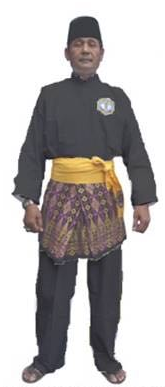
\includegraphics[height=2.5in]{images/chairperson}
        }
        ~
        \subfigure[Council of Referee-Jury]{\label{fig:council_wasit_juri}
            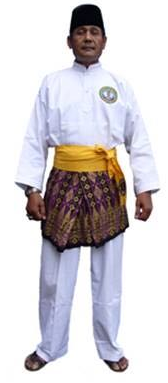
\includegraphics[height=2.5in]{images/council_wasit_juri}
        }
        ~
        \subfigure[Referee and Jury]{\label{fig:wasit_juri}
            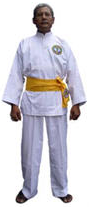
\includegraphics[height=2.5in]{images/wasit_juri}
        }
        ~
        \caption{Competition Officials}
    \end{figure}


\begin{legal}
\item Competition Chairperson
Competition Chairperson shall wear the standard BLACK PERSILAT Pencak Silat uniform 
(Figure~\ref{fig:committee_chairperson}) with:

    \begin{enumerate}[label=\alph*.]
    \item yellow `\emph{bengkung}' / sash 10 cm wide 
    \item `\emph{kain samping}' (traditional sarong-like adornment)
    \item a black `\emph{songkok}' hat.
    \end{enumerate}

At the left side of the chest is the badge of International Referee-Jury of PERSILAT
corresponding to the Chairperson's class. 

\item The Council of Referee-Jury

The Council of Referee-Jury for Tanding, Tunggal, Ganda and Regu categories shall wear the
standard WHITE PERSILAT Pencak Silat uniform (Figure~\ref{fig:council_wasit_juri}) with:

    \begin{enumerate}[label=\alph*.]
    \item yellow `\emph{bengkung}' / sash 10 cm wide 
    \item `\emph{kain samping}' (traditional sarong-like adornment)
    \item a black `\emph{songkok}' hat.
    \end{enumerate}

At the left side of the chest is the badge of International Referee-Jury of PERSILAT
according to Wasit's or Juri's class. 

\item Referee and Jury

Referee and Jury for Tanding, Tunggal, Ganda and Regu categories shall wear the 
standard WHITE PERSILAT Pencak Silat uniform

    \begin{enumerate}[label=\alph*.]
    \item yellow `\emph{bengkung}' / sash 10 cm wide 
    \end{enumerate}

At the left side of the chest is the badge of International Referee-Jury of PERSILAT
according to Wasit's or Juri's class. 

\item The Secretary, Assistant Secretary, Time Keeper and Arena Assistants. \\

Shall wear a uniform specified by the event Organizing Committee.

\end{legal}
